\documentclass[11pt,titlepage]{article}
\usepackage{ucs}
\usepackage[utf8x]{inputenc}
\usepackage[T1]{fontenc}
\usepackage[ngerman]{babel}
\usepackage{graphicx}
\usepackage{titlesec}
\usepackage{url}
\usepackage{lastpage}
\usepackage{listings}
\usepackage{color}
\usepackage{fancyhdr}
\usepackage{geometry}
\usepackage{wrapfig}
\usepackage{float}
\usepackage{subcaption}
\usepackage{hyperref}
\hypersetup{
    colorlinks=true,
    linkcolor=black,
    anchorcolor=black,
	citecolor=black,
	filecolor=black,
	menucolor=black,
	runcolor=black,
    urlcolor=blue,
	linktoc=all,
    pdftitle={Linux Networking},
    pdfauthor={Markus Gachnang und Martin Sprecher}
}
\usepackage{ragged2e}
\usepackage{framed}
\usepackage{quoting}
\usepackage{lscape}
\usepackage[table]{xcolor}
\usepackage{graphicx} 
\usepackage{pdfpages}
% remove current style and use fancyplain
\pagestyle{fancyplain}
\fancyhf{}
% remove rule/lines as well
\renewcommand{\headrulewidth}{0pt}
\renewcommand{\footrulewidth}{0pt}
% set papersize, magin and footersize
\geometry{a4paper,portrait,left={3cm},right={3cm},top={2cm},bottom={1cm},includefoot,foot={1cm}}
% set footer
\rfoot{Seite \thepage \hspace{1pt} von \pageref{LastPage}}
% Bibliographie
\usepackage{cite}
\def\BibTeX{{\rm B\kern-.05em{\sc i\kern-.025em b}\kern-.08em
    T\kern-.1667em\lower.7ex\hbox{E}\kern-.125emX}}
% define some colors
\definecolor{lightgray}{rgb}{.95,.95,.95}
\definecolor{shadecolor}{rgb}{.95,.95,.95}
\definecolor{darkgray}{rgb}{.4,.4,.4}
\definecolor{purple}{rgb}{0.65, 0.12, 0.82}
% set color and font of ''\url''
\renewcommand\UrlFont{\color{blue}\rmfamily\itshape}
% colorbox which can wrap lines
\newcommand\code[1]{\codehelp#1 \relax\relax}
\def\codehelp#1 #2\relax{\allowbreak\grayspace\codecolor{#1}\ifx\relax#2\else
 \codehelp#2\relax\fi}
\newcommand\codecolor[1]{\colorbox{lightgray}{\textcolor{black}{%
  \ttfamily\mystrut\smash{\detokenize{#1}}}}}
\def\mystrut{\rule[\dimexpr-\dp\strutbox+\fboxsep]{0pt}{%
 \dimexpr\normalbaselineskip-2\fboxsep}}
\def\grayspace{\hspace{0pt minus \fboxsep}}
% add ''\code'' to highligth single code lines
%\newcommand{\code}[1]{\wrapcolorbox[lightgray]{\ttfamily{#1}}}

% add ''\shadedquotation'' to highligth quoates
\newenvironment{shadedquotation}
 {\begin{shaded*}
  \quoting[leftmargin=0pt, vskip=0pt]
 }
 {\endquoting
 \end{shaded*}
}

% define ''JavaScript'' as a language for enviroment ''lstlisting''
\lstdefinelanguage{JavaScript}{
  keywords={typeof, new, true, false, catch, function, return, null, catch, switch, var, if, in, while, do, else, case, break},
  keywordstyle=\color{blue}\bfseries,
  ndkeywords={class, export, boolean, throw, implements, import, this},
  ndkeywordstyle=\color{darkgray}\bfseries,
  identifierstyle=\color{black},
  sensitive=false,
  comment=[l]{//},
  morecomment=[s]{/*}{*/},
  commentstyle=\color{purple}\ttfamily,
  stringstyle=\color{red}\ttfamily,
  morestring=[b]',
  morestring=[b]''
}

\lstset{
   language=JavaScript,
   backgroundcolor=\color{lightgray},
   extendedchars=true,
   basicstyle=\footnotesize\ttfamily,
   showstringspaces=false,
   showspaces=false,
   numbers=left,
   numberstyle=\footnotesize,
   numbersep=9pt,
   tabsize=2,
   breaklines=true,
   showtabs=false,
   captionpos=b
}
% set title
\title{Linux Networking}
\author{Markus Gachnang und Martin Sprecher}
\date{\today{}}
% set parindent to 0px to remove it (Einrücken von neuer Absatz)
\setlength\parindent{0pt}
% ---------------------------------------------------------------------------
% begin Document
\begin{document}
% set font
\sffamily
% print title
\maketitle
\newpage
% print index
\tableofcontents{}
\setcounter{page}{1}
\newpage
% linksbündig
\RaggedRight
% kein brechen von Wörtern
\tolerance=1
\emergencystretch=\maxdimen
\hyphenpenalty=10000
\hbadness=10000
% medskip before section
\let\SectionOriginal\section
\renewcommand\section[1]{\par\medskip\SectionOriginal{#1}}
% medskip before subsection
\let\SubSectionOriginal\subsection
\renewcommand\subsection[1]{\par\medskip\SubSectionOriginal{#1}}

\section{Flood and Learn}
\label{sec:FloodAndLearn}
This section contains the information in order to configure the virtualization technique VXLAN with the Flood and Learn approach.
In the following Figure you can see the topology of the network. The same topology is used in both use cases (flood and learn, evpn). However in the Flood and Learn approach only the
clients inside VLAN 140 are used.
\begin{figure}[H]
	\centering
	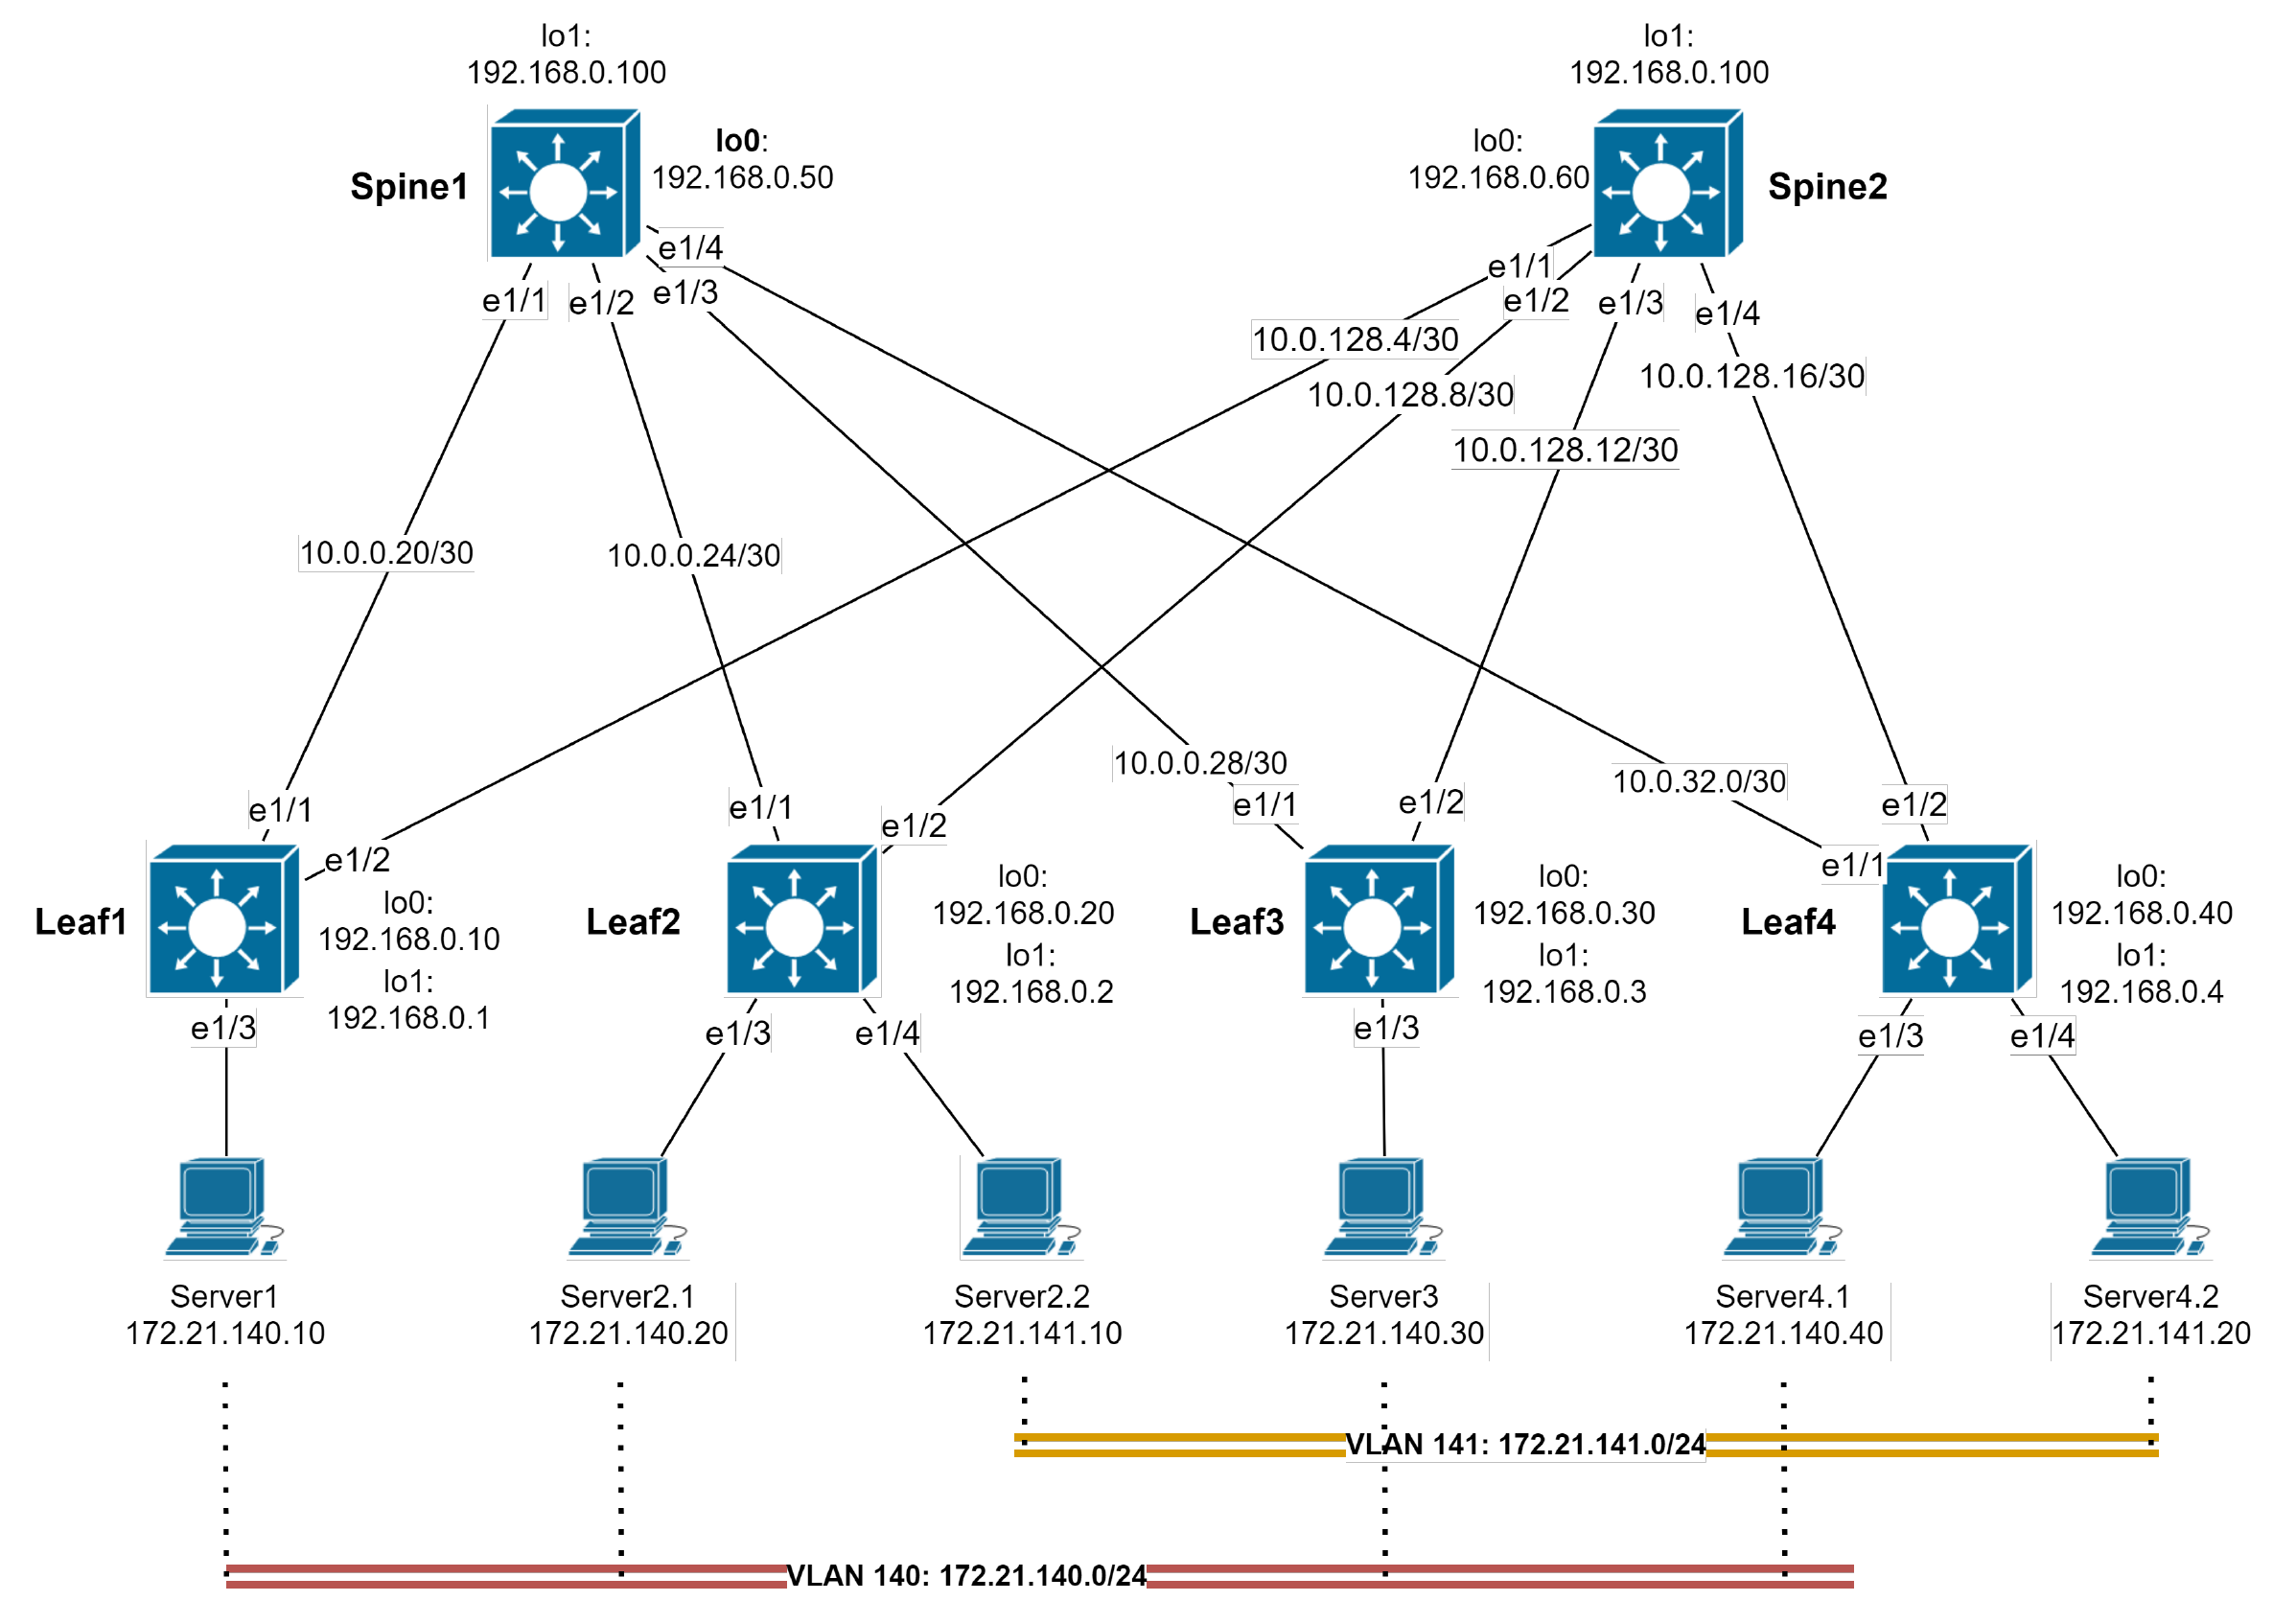
\includegraphics[width=0.9\linewidth]{images/topology}
	\caption{}
	\label{fig:topology}
\end{figure}
The goal is it that you enable the clients to ping between eachother. All traffic between the
clients shall be sent over the multicast-group used by the VTEPs.
The underlay connectivity between all interfaces drawn in the topology is already established.
As routing protocol OSPF is used and should work properly. You can check the OSPF configuration
by displaying all OSPF neighbors and pinging the interfaces. Each leaf should have both
spines as neighbors and the spines all leafes. Your job is it now to configure VXLAN. We will
provide step by step what you have to do but not how to configure it. So it’s your task to look
up the needed commands and should also be able to explain why that piece of configuration is needed. You don’t have to configure new interfaces or any underlay routing. That part of the
configuration is provided. The following steps shall be used as a guideline to implement VXLAN.

\begin{shadedquotation}
	\begin{enumerate}
		\item Configure Multicast: The first step is it to configure PIM-ASM with a rendez-vous point on the spine switches.
		\begin{itemize}
			\item use the spines loopback 1 as rendez-vous point
			\item configure Spine and Leaf interfaces for PIM
	\end{itemize}
		\item The next step will be the creation of the VLANs and the virtual network identifiers. The VNIs need to be linked to the VLANs. Use the VLAN-ID 140 and as VNI 50140.
		\item Now you have to create the VXLAN tunnel interfaces. Don’t forget to add the tunnel endpoints to the VNI and multicast group. All VTEPs in VLAN 140 should belong to the multicast-group 239.0.0.140.
  \end{enumerate}
\end{shadedquotation}

\subsection{Verification}
\label{subsec:Verification}
\begin{shadedquotation}
  Ping between the clients inside the VLAN 140.
  The following list contains commands which could be helpful while debugging/understanding   the configuration.
  \begin{itemize}
  	\item sh ip pim neighbor
  	\item sh ip mroute
  	\item sh nve peers
  	\item sh nve vni X
  	\item sh system internal l2fwder mac
  \end{itemize}
\end{shadedquotation}
\section{eVPN}
\subsection{Before you start}
In this chapter you will use the same topology with the hosts inside VLAN 141.
\subsection{EVPN Configuration}
You have already seen how VXLAN together with multicast allows us to expand a layer 2 domain over a routed core. Untill now we used one VLAN to connect multiple clients. In the new topology we will have two VLANs for the clients. The at the VTEPs learned client MAC addresses shall be propagated over BGP l2vpn evpn address-familiy updates to the Spine switches (functioning as route-reflectors). From there the updates will be sent to the other leave switches. This method called eVPN provides a very efficient way to propagate MAC addresses.
\begin{shadedquotation}
	Your configuration must fulfill the following conditions:
	\begin{itemize}
		\item Use VLAN 140 and 141 and the corresponding VNI 50140 and 50141 for the client L2
		domains.
		\item For the L3 routing in the core, use VLAN 999 with the VNI 50999.
		\item Use an isolated RIB (VRF) Tenant-1 and link it to the L3 VNI.
	\end{itemize}
\end{shadedquotation}
The following figure displays the same topology as in the Flood and Learn approach. In the EVPN configuration you will also enable the clients to ping between different VLANs, so you will use all servers.
\begin{figure}[H]
	\centering
	\includegraphics[width=0.9\linewidth]{"images/topology eVPN"}
	\caption{Network topology}
	\label{fig:topology-evpn}
\end{figure}
The following steps are needed to configure eVPN.
\begin{shadedquotation}
	\begin{enumerate}
		\item Create loopback 0 interfaces first as drawn in the topology. The interface will use a 32-bit subnetmask.
		\item Configure Anycast Multicast: The basic multicast configuration can be taken from the previous topology.
		\begin{itemize}
			\item On the spines add the configuration for anycast.
			\item On the leafes configure the anycast gateway MAC address.
		\end{itemize}
		\item Configure basic iBGP reachability: The Spine switches will act as route-reflectors to the Leaf switches. This will eliminate the requirement of a full-mesh peering. All leafes will be dual-homed to both spine switches.
		\begin{itemize}
			\item The whole network runs in AS 65000.
			\item Use the loopback 0 interfaces for peering
			\item Configure the route-reflectors.
			\item Allow standard and extended BGP communities to be exchanged with the neighbors
		\end{itemize}
		\item Configure VLANs: Configure the VLANs 140, 141 and 999. Don’t forget to assign the VNIs 	50140, 50141 or 50999 to the VLANs.
		\item Configure a VRF called Tenant-1 on the Leaf switches
		\begin{itemize}
			\item Link the VRF to the L3 VNI
			\item Inside the address-family ipv4 unicast define the rd, route-trarget import/export policies (because we use iBGP auto could be used). Do the same for evpn.
		\end{itemize}
		\item Configure the SVIs:
		\begin{itemize}
			\item Use the first IP address of each VLAN as the SVIs IP address
			\item Configure the SVIs as members of the created VRF
			\item Enable fabric distributed anycast-gateway (Hint: fabric forwarding mode ....)
		\end{itemize}
		\item Configure/adjust the NVE interface:
		\begin{itemize}
			\item Add all VNIs and their corresponding multicast-address/VRF
			\item Define BGP as mechanism for host reachability	
		\end{itemize}
		\item Configure EBGP EVPN control plane:
		\begin{itemize}
			\item Add the l2vpn evpn address-family and configure retain route-target all (This will except all updates containing any route-target). Under the address-family, allow standard and extended bgp communities.
		\end{itemize}
	\end{enumerate}
\end{shadedquotation}
\subsection{Verification}
In order to ping between the clients you need to open a ssh connection to the servers and enter
the ping command. In addition to the commands in section Flood and Learn the following could
also be helpful.
\begin{shadedquotation}
	\begin{itemize}
		\item sh ip bgp sum
		\item sh bgp ipv4 unicast summary
		\item sh bgp l2vpn evpn summary
		\item sh bgp l2vpn evpn summary
		\item sh l2route evpn mac-ip all
	\end{itemize}
\end{shadedquotation}
\subsection{Questions}
This chapter contains all questions you must answer for a successful delivery. Don’t forget to add
your configuration to the delivery!
\begin{shadedquotation}
	1. Compare the design with Flood\&Learn and the design with BGP eVPN. What do you 	think are the advantages and disadvantages of each control-plane approach (technical and non-technical)? Which solution for the control-plane would you recommend if a company would like to deploy VXLAN in their Datacenter? Justify your answer.
\end{shadedquotation}
\begin{shadedquotation}
	2. Copy a MP-BGP EVPN Route type 2 update with all the BGP attributes (using the show bgp l2vpn evpn x.x.x.x where x.x.x.x is an IP address) from the CLI into your documentation.
\end{shadedquotation}
\begin{shadedquotation}
	3. Modify your configuration in your lab in order to display a MP-BGP EVPN Route type 3 update. Copy a MP-BGP EVPN Route type 3 update with all the BGP attributes (using the show bgp l2vpn evpn x.x.x.x where x.x.x.x is an IP address) from the CLI into your
	documentation.
\end{shadedquotation}
\begin{shadedquotation}
	4. Modify your configuration in your lab in order to see a MP-BGP EVPN Route type 5 update. Copy a MP-BGP EVPN Route type 5 update with all the BGP attributes (using the show bgp l2vpn evpn x.x.x.x where x.x.x.x is an IP address) from the CLI into your documentation.
\end{shadedquotation}


\subsection{Quellennachweis}
\label{subsec:Quellennachweis}

\begingroup
% Remove Titles eg "Literatur"
\renewcommand{\section}[2]{}%
% Reminder: Recreate "SmartFactory.bll" when "citavi/citavi.bib" gets changed => run BibTeX ([F11] in TexMaker)
\bibliography{Lab3_Quellen/quellen}
% Use the "IEEE standard" as style => "IEEEtran.bst"
\bibliographystyle{IEEEtran}
\endgroup  

\end{document}
